
%% bare_jrnl.tex
%% V1.3
%% 2007/01/11
%% by Michael Shell
%% see http://www.michaelshell.org/
%% for current contact information.
%%
%% This is a skeleton file demonstrating the use of IEEEtran.cls
%% (requires IEEEtran.cls version 1.7 or later) with an IEEE journal paper.
%%
%% Support sites:
%% http://www.michaelshell.org/tex/ieeetran/
%% http://www.ctan.org/tex-archive/macros/latex/contrib/IEEEtran/
%% and
%% http://www.ieee.org/


\documentclass[journal]{IEEEtran}
\usepackage{blindtext}
\usepackage{graphicx}
\usepackage{float}


% Some very useful LaTeX packages include:
% (uncomment the ones you want to load)

% Code syntax

\usepackage{listings}
\usepackage{color}

\definecolor{dkgreen}{rgb}{0,0.6,0}
\definecolor{gray}{rgb}{0.5,0.5,0.5}
\definecolor{mauve}{rgb}{0.58,0,0.82}

\lstset{frame=tb,
  language=C++,
  aboveskip=3mm,
  belowskip=3mm,
  showstringspaces=false,
  columns=flexible,
  basicstyle={\small\ttfamily},
  numbers=none,
  numberstyle=\tiny\color{gray},
  keywordstyle=\color{blue},
  commentstyle=\color{dkgreen},
  stringstyle=\color{mauve},
  breaklines=true,
  breakatwhitespace=true
  tabsize=2
}

% \setlength{\columnsep}{0.5in}
% \setlength{\columnseprule}{1px}

% *** MISC UTILITY PACKAGES ***
%
%\usepackage{ifpdf}
% Heiko Oberdiek's ifpdf.sty is very useful if you need conditional
% compilation based on whether the output is pdf or dvi.
% usage:
% \ifpdf
%   % pdf code
% \else
%   % dvi code
% \fi
% The latest version of ifpdf.sty can be obtained from:
% http://www.ctan.org/tex-archive/macros/latex/contrib/oberdiek/
% Also, note that IEEEtran.cls V1.7 and later provides a builtin
% \ifCLASSINFOpdf conditional that works the same way.
% When switching from latex to pdflatex and vice-versa, the compiler may
% have to be run twice to clear warning/error messages.


% *** CITATION PACKAGES ***
%

\usepackage{cite}

% *** GRAPHICS RELATED PACKAGES ***
%
\ifCLASSINFOpdf
  % \usepackage[pdftex]{graphicx}
  % declare the path(s) where your graphic files are
  % \graphicspath{{../pdf/}{../jpeg/}}
  % and their extensions so you won't have to specify these with
  % every instance of \includegraphics
  % \DeclareGraphicsExtensions{.pdf,.jpeg,.png}
\else
  % or other class option (dvipsone, dvipdf, if not using dvips). graphicx
  % will default to the driver specified in the system graphics.cfg if no
  % driver is specified.
  % \usepackage[dvips]{graphicx}
  % declare the path(s) where your graphic files are
  % \graphicspath{{../eps/}}
  % and their extensions so you won't have to specify these with
  % every instance of \includegraphics
  % \DeclareGraphicsExtensions{.eps}
\fi
% graphicx was written by David Carlisle and Sebastian Rahtz. It is
% required if you want graphics, photos, etc. graphicx.sty is already
% installed on most LaTeX systems. The latest version and documentation can
% be obtained at:
% http://www.ctan.org/tex-archive/macros/latex/required/graphics/
% Another good source of documentation is "Using Imported Graphics in
% LaTeX2e" by Keith Reckdahl which can be found as epslatex.ps or
% epslatex.pdf at: http://www.ctan.org/tex-archive/info/
%
% latex, and pdflatex in dvi mode, support graphics in encapsulated
% postscript (.eps) format. pdflatex in pdf mode supports graphics
% in .pdf, .jpeg, .png and .mps (metapost) formats. Users should ensure
% that all non-photo figures use a vector format (.eps, .pdf, .mps) and
% not a bitmapped formats (.jpeg, .png). IEEE frowns on bitmapped formats
% which can result in "jaggedy"/blurry rendering of lines and letters as
% well as large increases in file sizes.
%
% You can find documentation about the pdfTeX application at:
% http://www.tug.org/applications/pdftex





% *** MATH PACKAGES ***


\usepackage[cmex10]{amsmath}


% A popular package from the American Mathematical Society that provides
% many useful and powerful commands for dealing with mathematics. If using
% it, be sure to load this package with the cmex10 option to ensure that
% only type 1 fonts will utilized at all point sizes. Without this option,
% it is possible that some math symbols, particularly those within
% footnotes, will be rendered in bitmap form which will result in a
% document that can not be IEEE Xplore compliant!
%
% Also, note that the amsmath package sets \interdisplaylinepenalty to 10000
% thus preventing page breaks from occurring within multiline equations. Use:
%\interdisplaylinepenalty=2500
% after loading amsmath to restore such page breaks as IEEEtran.cls normally
% does. amsmath.sty is already installed on most LaTeX systems. The latest
% version and documentation can be obtained at:
% http://www.ctan.org/tex-archive/macros/latex/required/amslatex/math/





% *** SPECIALIZED LIST PACKAGES ***
%
%\usepackage{algorithmic}
% algorithmic.sty was written by Peter Williams and Rogerio Brito.
% This package provides an algorithmic environment fo describing algorithms.
% You can use the algorithmic environment in-text or within a figure
% environment to provide for a floating algorithm. Do NOT use the algorithm
% floating environment provided by algorithm.sty (by the same authors) or
% algorithm2e.sty (by Christophe Fiorio) as IEEE does not use dedicated
% algorithm float types and packages that provide these will not provide
% correct IEEE style captions. The latest version and documentation of
% algorithmic.sty can be obtained at:
% http://www.ctan.org/tex-archive/macros/latex/contrib/algorithms/
% There is also a support site at:
% http://algorithms.berlios.de/index.html
% Also of interest may be the (relatively newer and more customizable)
% algorithmicx.sty package by Szasz Janos:
% http://www.ctan.org/tex-archive/macros/latex/contrib/algorithmicx/




% *** ALIGNMENT PACKAGES ***
%
%\usepackage{array}
% Frank Mittelbach's and David Carlisle's array.sty patches and improves
% the standard LaTeX2e array and tabular environments to provide better
% appearance and additional user controls. As the default LaTeX2e table
% generation code is lacking to the point of almost being broken with
% respect to the quality of the end results, all users are strongly
% advised to use an enhanced (at the very least that provided by array.sty)
% set of table tools. array.sty is already installed on most systems. The
% latest version and documentation can be obtained at:
% http://www.ctan.org/tex-archive/macros/latex/required/tools/


%\usepackage{mdwmath}
%\usepackage{mdwtab}
% Also highly recommended is Mark Wooding's extremely powerful MDW tools,
% especially mdwmath.sty and mdwtab.sty which are used to format equations
% and tables, respectively. The MDWtools set is already installed on most
% LaTeX systems. The lastest version and documentation is available at:
% http://www.ctan.org/tex-archive/macros/latex/contrib/mdwtools/


% IEEEtran contains the IEEEeqnarray family of commands that can be used to
% generate multiline equations as well as matrices, tables, etc., of high
% quality.


%\usepackage{eqparbox}
% Also of notable interest is Scott Pakin's eqparbox package for creating
% (automatically sized) equal width boxes - aka "natural width parboxes".
% Available at:
% http://www.ctan.org/tex-archive/macros/latex/contrib/eqparbox/


\usepackage{subcaption}



% *** SUBFIGURE PACKAGES ***
% \usepackage[tight,footnotesize]{subfigure}
% subfigure.sty was written by Steven Douglas Cochran. This package makes it
% easy to put subfigures in your figures. e.g., "Figure 1a and 1b". For IEEE
% work, it is a good idea to load it with the tight package option to reduce
% the amount of white space around the subfigures. subfigure.sty is already
% installed on most LaTeX systems. The latest version and documentation can
% be obtained at:
% http://www.ctan.org/tex-archive/obsolete/macros/latex/contrib/subfigure/
% subfigure.sty has been superceeded by subfig.sty.



% \usepackage[caption=false]{caption}
% \usepackage[font=footnotesize]{subfig}
% subfig.sty, also written by Steven Douglas Cochran, is the modern
% replacement for subfigure.sty. However, subfig.sty requires and
% automatically loads Axel Sommerfeldt's caption.sty which will override
% IEEEtran.cls handling of captions and this will result in nonIEEE style
% figure/table captions. To prevent this problem, be sure and preload
% caption.sty with its "caption=false" package option. This is will preserve
% IEEEtran.cls handing of captions. Version 1.3 (2005/06/28) and later
% (recommended due to many improvements over 1.2) of subfig.sty supports
% the caption=false option directly:
%\usepackage[caption=false,font=footnotesize]{subfig}
%
% The latest version and documentation can be obtained at:
% http://www.ctan.org/tex-archive/macros/latex/contrib/subfig/
% The latest version and documentation of caption.sty can be obtained at:
% http://www.ctan.org/tex-archive/macros/latex/contrib/caption/



% *** FLOAT PACKAGES ***
%
%\usepackage{fixltx2e}
% fixltx2e, the successor to the earlier fix2col.sty, was written by
% Frank Mittelbach and David Carlisle. This package corrects a few problems
% in the LaTeX2e kernel, the most notable of which is that in current
% LaTeX2e releases, the ordering of single and double column floats is not
% guaranteed to be preserved. Thus, an unpatched LaTeX2e can allow a
% single column figure to be placed prior to an earlier double column
% figure. The latest version and documentation can be found at:
% http://www.ctan.org/tex-archive/macros/latex/base/



%\usepackage{stfloats}
% stfloats.sty was written by Sigitas Tolusis. This package gives LaTeX2e
% the ability to do double column floats at the bottom of the page as well
% as the top. (e.g., "\begin{figure*}[!b]" is not normally possible in
% LaTeX2e). It also provides a command:
%\fnbelowfloat
% to enable the placement of footnotes below bottom floats (the standard
% LaTeX2e kernel puts them above bottom floats). This is an invasive package
% which rewrites many portions of the LaTeX2e float routines. It may not work
% with other packages that modify the LaTeX2e float routines. The latest
% version and documentation can be obtained at:
% http://www.ctan.org/tex-archive/macros/latex/contrib/sttools/
% Documentation is contained in the stfloats.sty comments as well as in the
% presfull.pdf file. Do not use the stfloats baselinefloat ability as IEEE
% does not allow \baselineskip to stretch. Authors submitting work to the
% IEEE should note that IEEE rarely uses double column equations and
% that authors should try to avoid such use. Do not be tempted to use the
% cuted.sty or midfloat.sty packages (also by Sigitas Tolusis) as IEEE does
% not format its papers in such ways.


% *** PDF, URL AND HYPERLINK PACKAGES ***
%
%\usepackage{url}
% url.sty was written by Donald Arseneau. It provides better support for
% handling and breaking URLs. url.sty is already installed on most LaTeX
% systems. The latest version can be obtained at:
% http://www.ctan.org/tex-archive/macros/latex/contrib/misc/
% Read the url.sty source comments for usage information. Basically,
% \url{my_url_here}.





% *** Do not adjust lengths that control margins, column widths, etc. ***
% *** Do not use packages that alter fonts (such as pslatex).         ***
% There should be no need to do such things with IEEEtran.cls V1.6 and later.
% (Unless specifically asked to do so by the journal or conference you plan
% to submit to, of course. )


% correct bad hyphenation here
\hyphenation{op-tical net-works semi-conduc-tor a-ppli-ed}


\begin{document}
%
% paper title
% can use linebreaks \\ within to get better formatting as desired
\title{Counting taxis with automatic tracking.}
%
%
% author names and IEEE memberships
% note positions of commas and nonbreaking spaces ( ~ ) LaTeX will not break
% a structure at a ~ so this keeps an author's name from being broken across
% two lines.
% use \thanks{} to gain access to the first footnote area
% a separate \thanks must be used for each paragraph as LaTeX2e's \thanks
% was not built to handle multiple paragraphs
%

\author{
  Manuel~Felipe~Pineda~Loaiza,
  ~\IEEEmembership{MSc. Student,~Universidad Tecnológica de Pereira}
}


% note the % following the last \IEEEmembership and also \thanks -
% these prevent an unwanted space from occurring between the last author name
% and the end of the author line. i.e., if you had this:
%
% \author{....lastname \thanks{...} \thanks{...} }
%                     ^------------^------------^----Do not want these spaces!
%
% a space would be appended to the last name and could cause every name on that
% line to be shifted left slightly. This is one of those "LaTeX things". For
% instance, "\textbf{A} \textbf{B}" will typeset as "A B" not "AB". To get
% "AB" then you have to do: "\textbf{A}\textbf{B}"
% \thanks is no different in this regard, so shield the last } of each \thanks
% that ends a line with a % and do not let a space in before the next \thanks.
% Spaces after \IEEEmembership other than the last one are OK (and needed) as
% you are supposed to have spaces between the names. For what it is worth,
% this is a minor point as most people would not even notice if the said evil
% space somehow managed to creep in.



% The paper headers
\markboth{Computer vision class, Universidad Tecnologica de Pereira ~ 2017-II}%
{Shell \MakeLowercase{\textit{et al.}}: Bare Demo of IEEEtran.cls for Journals}


% make the title area
\maketitle


\begin{abstract}
%\boldmath
This work covers the problem of detection and tracking of moving objects in a
video with the specific goal of counting taxis. In this work we used computer
vision techniques such background subtraction, segmentation and tracking with
the help of OpenCV and python 3.
\end{abstract}

% Note that keywords are not normally used for peerreview papers.
\begin{IEEEkeywords}
Computer vision, background subtraction, segmentation, kalman filter, OpenCV.
\end{IEEEkeywords}

\section{Introduction}


The video tracking is the process of locating a moving object over the time.
It has a bast field of applications, some of which are \cite{wiki:tracking}:
video-surveillance, augmented reality, and traffic control.

The goal of the video tracking is to associate target objects in consecutive
frames of the video. This is a complex task because it depends on several
factors that change with the time, some of them are, for example:
the trajectory of the objects and the illumination on the scene. For this
reason the problem is divided in several stages that will be described later.
The big picture of the process is:

\begin{enumerate}
  \item Subtract background.
  \item Image Segmentation / Classification.
  \item Tracking.
  \item Counting.
\end{enumerate}


\section{Process}

\subsection{Color filter and background subtraction}

In the background subtraction stage we take the original video as input and
we classify each pixel as either background or foreground for further analysis
(object detection and tracking). We initially used the OpenCV method
\texttt{createBackgroundSubtractorMOG2} which internally uses a Mixture Of
Gaussians. This worked well but we had to tune the \texttt{threshold} because
the filter was very noisy and was not so stable with the illumination changes.

In order to improve that, we applied a color filter before the background
subtraction task, this helped a lot with the noise in the background and it was
also beneficial for the classification stage since in the video the only yellow
vehicles were in fact the taxis. In the figure \ref{background-comp} we show
the comparison between the background subtraction without the color filter
and with the color filter.

To do this color filtering, we defined a color space for the ``yellow'' and
filtered out all the pixels who where not in the color space. The figure
\ref{color-filter} shows the result of the color filter.


\begin{figure}
  \centering
  \begin{subfigure}[b]{0.2\textwidth}
  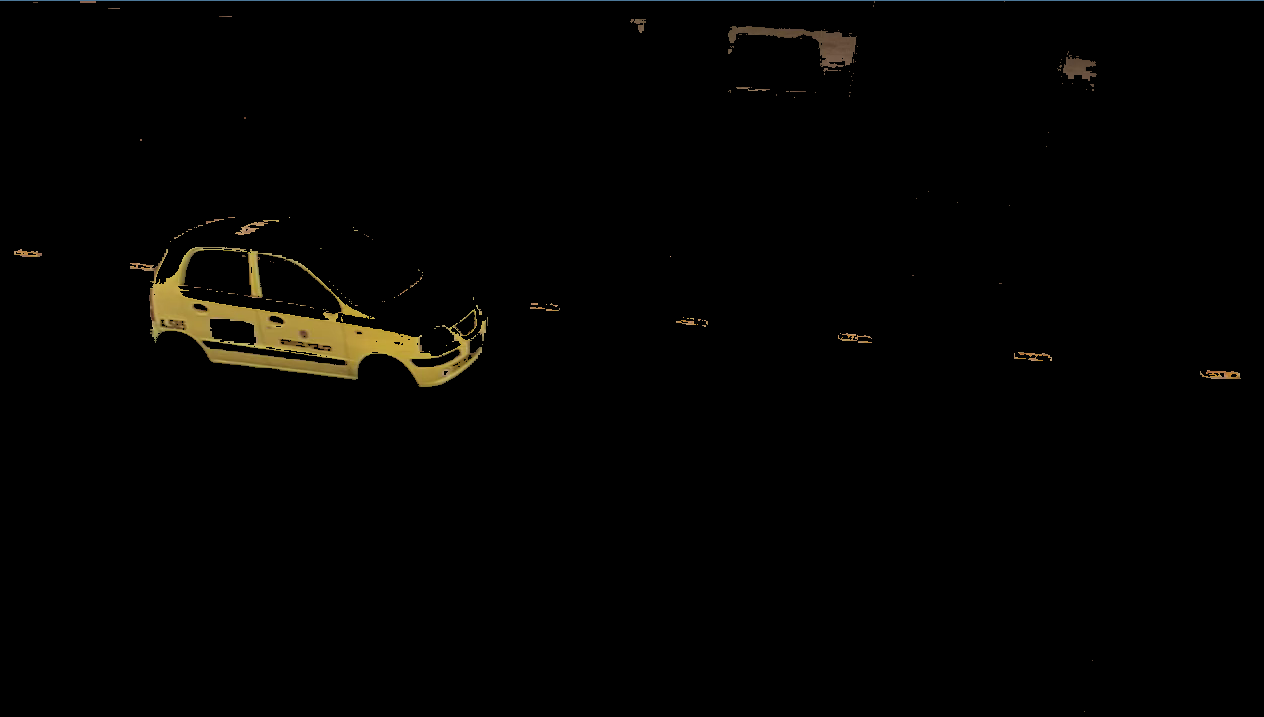
\includegraphics[scale=0.09]{../img/yellow}
  \caption{Color filter.}
  \end{subfigure}
  ~ %add desired spacing between images, e. g. ~, \quad, \qquad, \hfill etc.
  %(or a blank line to force the subfigure onto a new line)
  \begin{subfigure}[b]{0.2\textwidth}
  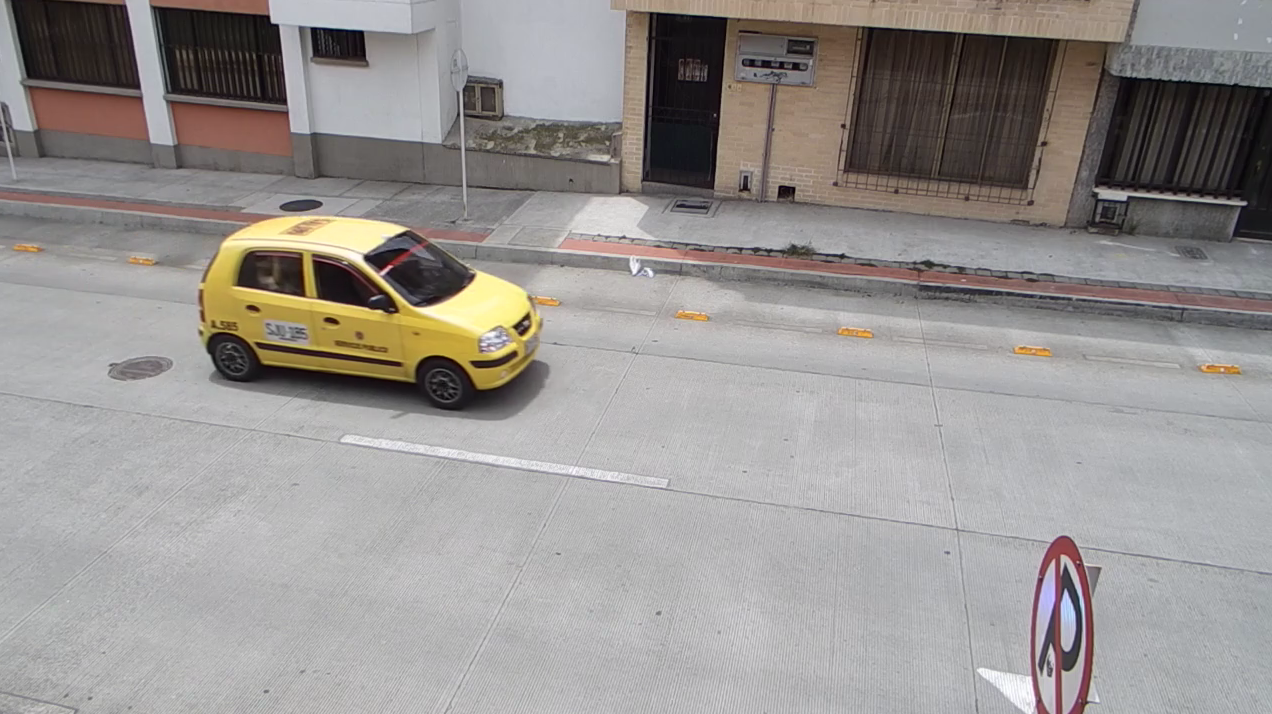
\includegraphics[scale=0.09]{../img/original}
  \caption{Original image.}
  \end{subfigure}
  \caption{Color filter applied to the original image}
  \label{color-filter}
\end{figure}

\begin{figure}
  \centering
  \begin{subfigure}[b]{0.2\textwidth}
  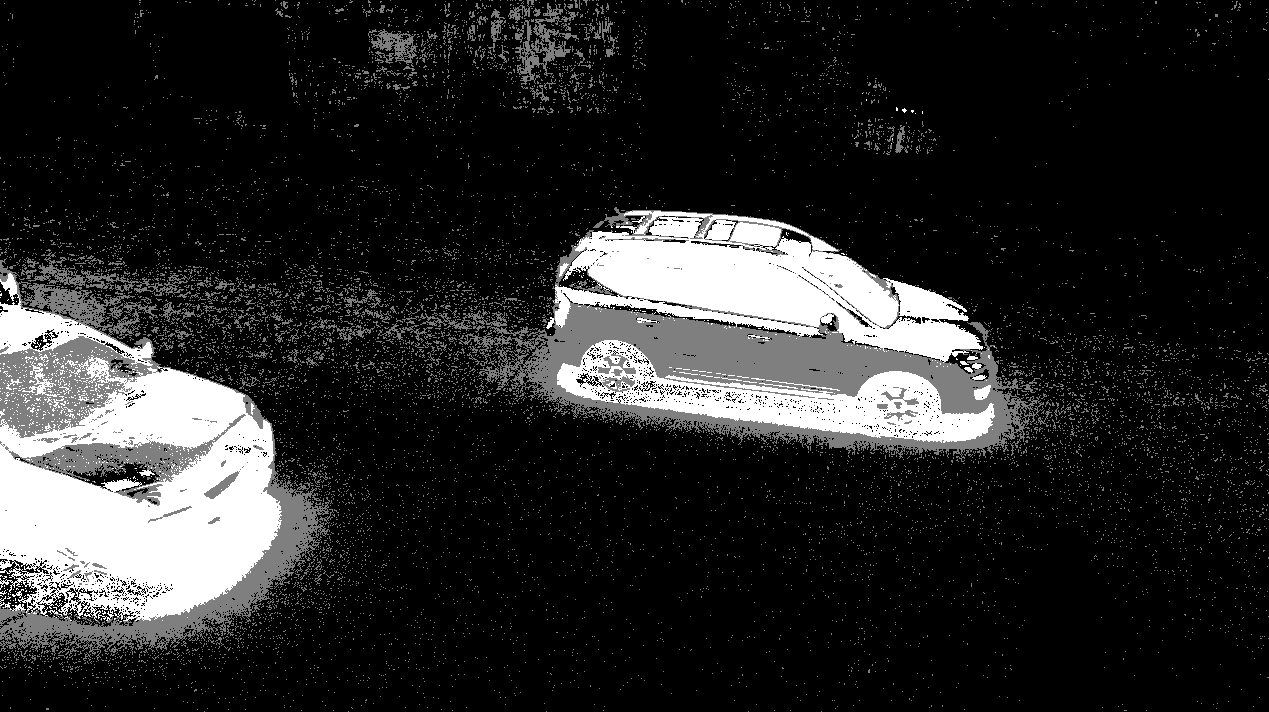
\includegraphics[scale=0.09]{../img/noisy}
  \caption{Noisy background subtraction.}
  \end{subfigure}
  ~ %add desired spacing between images, e. g. ~, \quad, \qquad, \hfill etc.
  %(or a blank line to force the subfigure onto a new line)
  \begin{subfigure}[b]{0.2\textwidth}
  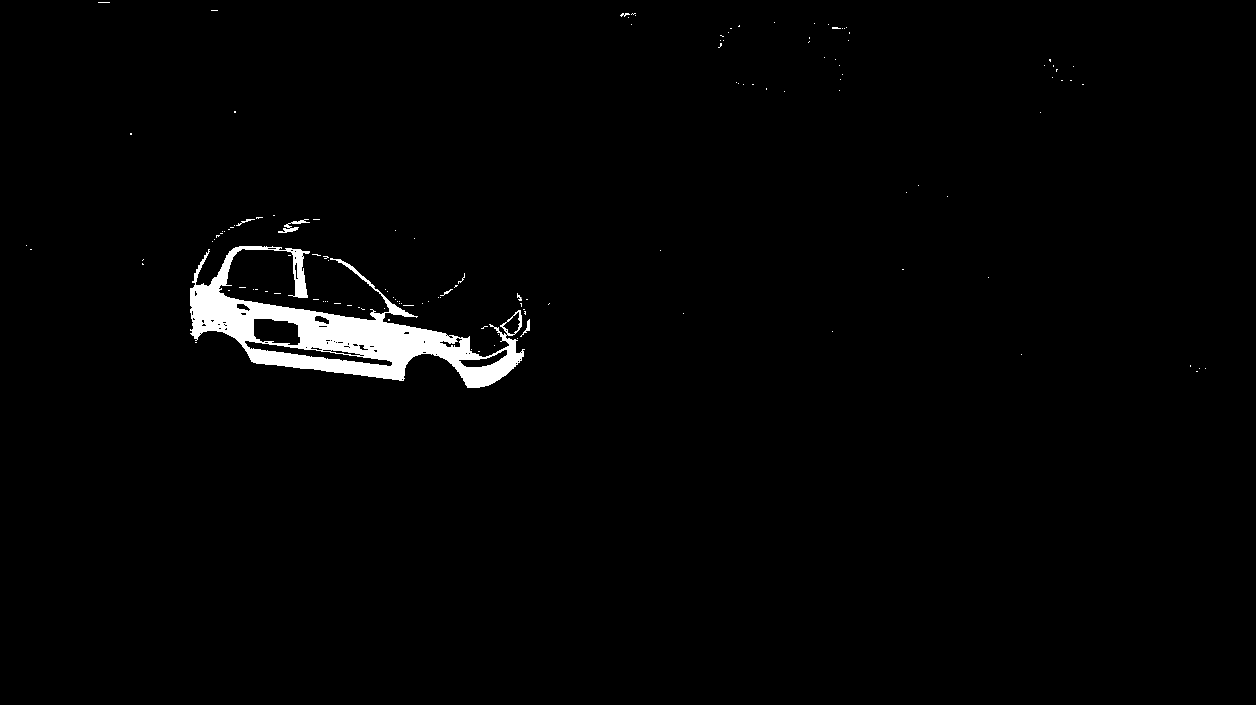
\includegraphics[scale=0.09]{../img/background}
  \caption{background subtraction after color filter.}
  \end{subfigure}
  \caption{background subtraction comparison's}
  \label{background-comp}
\end{figure}



\subsection{Segmentation}

The goal of this stage is to separate the objects in the image, in our particular
case, is in charge of detecting the taxis. To achieve this we found the contours
in the image using the method \texttt{findContours} of OpenCV. For each image,
we filtered out all the contours that were too small o too large based in the
``normal'' size of a car in the image. Each contour is described as a bounding
box around the taxi, only the valid contours are passed to the next stage.

Usually, some machine-learning related techniques are applied at this point
to improve the detection and classification of the objects in the image.
However in our case that was not necessary because the color and the size
were really good descriptors of the taxis.

\subsection{Tracking}

Given the contour (bounding box) of the taxi we computed the central points
\cite{opencv:moments} and we used them as the position of the taxi. With the 
position of the taxi in each frame, we used a Kalman filter to estimate
the real position of the vehicle.

The kalman filter is an optimal recursive Bayesian filter for linear functions
subjected to Gaussian noise \cite{wiki:kalman}. The goal of this filter is to 
generate precise estimations over the time. It is composed by two equations:

\begin{equation}
  x_{k} = Ax_{k - 1} + w_{k - 1}
\end{equation}

Where $x_{k}$ is the state vector at time $k$, $A$ is the transition matrix
and $w_{k - 1}$ is the process noise.


\begin{equation}
  z_{k} = Hx_{k} + v_{k}
\end{equation}

Where $z_{k}$ is the measurement itself, $H$ is a matrix that maps the state to 
the measurement, and $v_{k}$ is the measurement noise.

We modeled the Kalman filter for a 2D motion with
constant speed.

\begin{equation}
  px_{k} = px_{k - 1} + {\Delta}t * vx
\end{equation}

\begin{equation}
  py_{k} = py_{k - 1} + {\Delta}t * vy
\end{equation}

Where $px_{k}$ and $py_{k}$  is the position in $x, y$ at the time $k$ and
$vx_{k}$ and $vy_{k}$ are the components of the speed. Then we can define a state
vector as:

\begin{equation}
  x = 
  \begin{bmatrix}
      px \\
      py \\
      vx \\
      vy
  \end{bmatrix}
\end{equation}

And the transition matrix is:

\begin{equation}
  A =
  \begin{bmatrix}
      1 & 0 & {\Delta}t & 0 \\
      0 & 1 & 0 & {\Delta}t \\
      0 & 0 & 1 & 0 \\
      0 & 0 & 0 & 1
  \end{bmatrix}
\end{equation}

And finally the measure matrix is:

\begin{equation}
  H =
  \begin{bmatrix}
      1 & 0 & 0 & 0 \\
      0 & 1 & 0 & 0 \\
  \end{bmatrix}
\end{equation}

For the implementation of this stage we used OpenCV with the model described
above.

\subsection{Counting}

This stage is really simple and it was merged with the tracking in the code,
basically when a predefined threshold is passed between two measurements of the
position, we count the object as a new taxi and we reset all the parameters
of the filter.

\begin{figure}[H]
  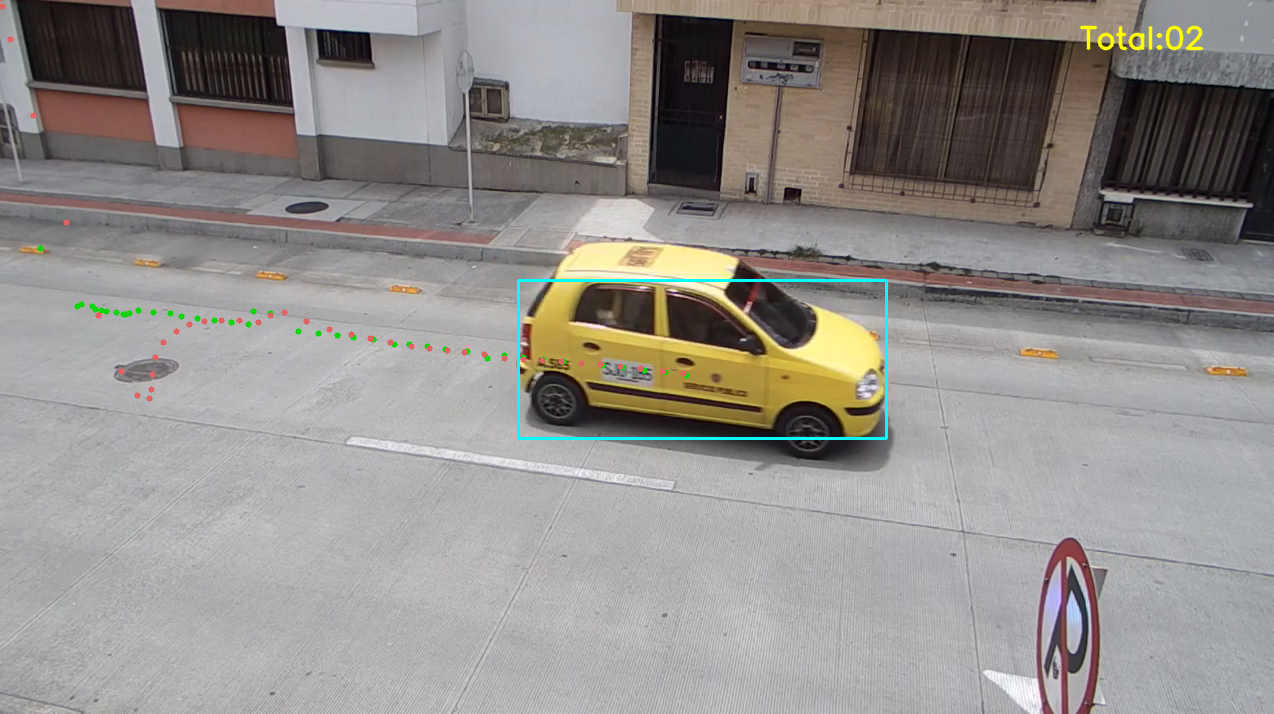
\includegraphics[scale=0.2]{../img/counting}
  \caption{Final output of the tracking and counting.}
  \label{final}
\end{figure}

\section{Experiments and results.}

All the images shown in the report were generated by our code. The test videos
were taken using a Fujifilm Finepix SL1000 camera.

In the tested video, the accuracy of counting the taxis was of the 100\% but
we still have an unsolved problem which is the classification of yellow cars that
are not taxis.

\section{Conclusions}

The process of tracking and counting taxis in a video under normal conditions
of illumination and traffic worked as expected.

All the tuning of the parameters was done manually, this is a good starting
point for future work, merging this with more sophisticated techniques and
machine learning.

The background subtraction stage is a really complicated process, in this
case the color filter was a really good help but it not generalize to the
process of counting any type of vehicles.

\bibliographystyle{unsrt}
\bibliography{report}

% that's all folks
\end{document}
